%%%%%%%%%%%%%%%%%%%%%%%%%%%%%%%%%%%%%%%%%
% Beamer Presentation
% LaTeX Template
% Version 1.0 (10/11/12)
%
% This template has been downloaded from:
% http://www.LaTeXTemplates.com
%
% License:
% CC BY-NC-SA 3.0 (http://creativecommons.org/licenses/by-nc-sa/3.0/)
%
%%%%%%%%%%%%%%%%%%%%%%%%%%%%%%%%%%%%%%%%%

%----------------------------------------------------------------------------------------
%	PACKAGES AND THEMES
%----------------------------------------------------------------------------------------

\documentclass{beamer}

\mode<presentation> {

% The Beamer class comes with a number of default slide themes
% which change the colors and layouts of slides. Below this is a list
% of all the themes, uncomment each in turn to see what they look like.

%\usetheme{default}
%\usetheme{AnnArbor}
%\usetheme{Antibes}
%\usetheme{Bergen}
%\usetheme{Berkeley}
%\usetheme{Berlin}
%\usetheme{Boadilla}
%\usetheme{CambridgeUS}
%\usetheme{Copenhagen}
%\usetheme{Darmstadt}
%\usetheme{Dresden}
%\usetheme{Frankfurt}
%\usetheme{Goettingen}
%\usetheme{Hannover}
%\usetheme{Ilmenau}
%\usetheme{JuanLesPins}
%\usetheme{Luebeck}
\usetheme{Madrid}
%\usetheme{Malmoe}
%\usetheme{Marburg}
%\usetheme{Montpellier}
%\usetheme{PaloAlto}
%\usetheme{Pittsburgh}
%\usetheme{Rochester}
%\usetheme{Singapore}
%\usetheme{Szeged}
%\usetheme{Warsaw}

% As well as themes, the Beamer class has a number of color themes
% for any slide theme. Uncomment each of these in turn to see how it
% changes the colors of your current slide theme.

%\usecolortheme{albatross}
%\usecolortheme{beaver}
%\usecolortheme{beetle}
%\usecolortheme{crane}
%\usecolortheme{dolphin}
%\usecolortheme{dove}
%\usecolortheme{fly}
%\usecolortheme{lily}
%\usecolortheme{orchid}
%\usecolortheme{rose}
%\usecolortheme{seagull}
%\usecolortheme{seahorse}
%\usecolortheme{whale}
%\usecolortheme{wolverine}

%\setbeamertemplate{footline} % To remove the footer line in all slides uncomment this line
%\setbeamertemplate{footline}[page number] % To replace the footer line in all slides with a simple slide count uncomment this line

%\setbeamertemplate{navigation symbols}{} % To remove the navigation symbols from the bottom of all slides uncomment this line
}

\usepackage{graphicx} % Allows including images
\usepackage{booktabs} % Allows the use of \toprule, \midrule and \bottomrule in tables
\usepackage{verbatim}

%----------------------------------------------------------------------------------------
%	TITLE PAGE
%----------------------------------------------------------------------------------------

\title[Open Aircraft Design]{Open Source Aircraft Design} % The short title appears at the bottom of every slide, the full title is only on the title page

\author{Niel Agenbag} % Your name
\institute[Unaffiliated] % Your institution as it will appear on the bottom of every slide, may be shorthand to save space
{
Unaffiliated \\ % Your institution for the title page
\medskip
\textit{Ludwigprandtlwing@gmail.com} % Your email address
}
\date{\today} % Date, can be changed to a custom date

\begin{document}

\begin{frame}
\titlepage % Print the title page as the first slide
\end{frame}

\begin{frame}
\frametitle{Overview} % Table of contents slide, comment this block out to remove it
\tableofcontents % Throughout your presentation, if you choose to use \section{} and \subsection{} commands, these will automatically be printed on this slide as an overview of your presentation
\end{frame}

%----------------------------------------------------------------------------------------
%	PRESENTATION SLIDES
%----------------------------------------------------------------------------------------

\section{Introduction}

%------------------------------------------------

\begin{frame}
\frametitle{Find out more}

Find out more at the following accounts:

\begin{itemize}
\item youtube:  https://www.youtube.com/channel/UC6F9yife2uQ-U4vDy8oB4gA
\item github:  https://github.com/ludwigprandtlwing
\item instagram:  ludwigprandtlwing
\end{itemize}
\end{frame}

%------------------------------------------------

\begin{frame}
\frametitle{Introduction}

\begin{itemize}
\item Working with the Prandtl wing has highlighted the need for new ways of developing an aircraft.
\item This is made possible by broad changes as a result of mainly internet connectivity and the free software movements.
\item Open source engineering might be the solution
\end{itemize}

\end{frame}


\begin{frame}
\frametitle{Why Open Source}

New ways of doing engineering is required:

\begin{itemize}
\item Cost has to be reduced and open source provides free alternatives.
\item Innovation requires a framework and open source might fit the bill.
\item Open source engineering could be conducive to innovation because of its networked collaborative approach.
\end{itemize}
        
\end{frame}
        


\begin{frame}
\frametitle{Introduction:  Aircraft specific topics}

\begin{itemize}
\item Aircraft design requires specialist knowledge and skills  
\item Large capital investment is required, often with little guarantee of return on investment and often at low marginsconnectivity and the free software movements.
\item Things have changed though, with remotely piloted vehicles that can reduce risk, open source software, first person view, collaboration tools (GIT)
\end{itemize}

\end{frame}



\begin{comment}
Aircraft design requires specialist knowledge and skills.  Furthermore large capital investment is required, often with little guarantee of return on investment and often at low margins.  Things have changed though, with remotely piloted vehicles that can reduce risk, open source software, first person view, collaboration tools (GIT). \\~\\

Doing what hobbyists have been doing for years, exchanging components and expertise, but over the internet that facilitates the scaling of the design and analysis process.

Building and making tools
Distributing these tools
Creating a community of enthusiasts and professionals and connecting these individuals on a platform such as Github

Make it possible to commit CAD files via Python scripting

Enable trade of skills and equipment in an open way.

This removes the hysteresis (marketing department, sales, HR) associated with companies with large overheads.  Projects can easily spend money but bringing money in is difficult.
Pure trade (classical horse trading) immediately negates the losses associated with the existing system.
\end{comment}



\section{Requirements for networked innovation} 

\begin{frame}
\frametitle{Networked innovation}

\begin{itemize}
\item Metcalfe's law states the effect of a telecommunications network is proportional to the square of the number of connected users of the system ($n^2$) (from Wikipedia)
\item It is proposed that open sourced innovation and engineering on a suitably sophisticated platform with a sufficient number of users could have far reaching implications for high technology engineering because of the scaling principle.
\item Translated this means:  Get many people in a network working on your aircraft and you can get it done in a reasonable time.        
\end{itemize}

\end{frame}



\begin{frame}
\frametitle{Requirements for networked innovation}

The following seems to be necessary for this kind of innovation/product development

\begin{itemize}
\item Connectivity - internet
\item A local, enthusiastic group of individuals that can share and brainstorm ideas % This seems to be a prerequisite otherwise projects quickly loose momentum.  Typically this requires people in very close proximity such as an office or a small community, otherwise easy access in a city.
\item A broader community of individuals willing to contribute
\item An innovation framework - Guidelines on how the project is conducted:  Typically a document describing the methodologies used
\item A set of Free Open Soure Software (FOSS) tools
\item No restrictions on information - therefore open hardware and NO RESTRICTIVE PATENTS
\end{itemize}
\end{frame}


\section{FOSS Tools}

%------------------------------------------------

\begin{frame}
\frametitle{Bullet Points}

Many tools are required for designing, analysing and building an aircraft.  The following typical tools are required.  A libre, open source example of each is presented next to the type of software.

\begin{itemize}
\item Computer aided design (CAD) tools - FreeCAD
\item Finite element analysis - Calculix (bundled with FreeCAD) or Nastran95, Code Aster
\item Computational fluid dynamics (CFD) - OpenFOAM (also integrated with FreeCAD)
\item Rigid body dynamic simulation - Project Chrono
\item General matrix computation, large data processing for flight testing - Python
\item Version control - Git
\item Product lifecycle management - Combination of Git and a browser based framework such as Django (not yet developed, but envisaged)
\end{itemize}
\end{frame}

\begin{frame}
\frametitle{CAD}

CAD model of the Prandtl wing

\begin{figure}
        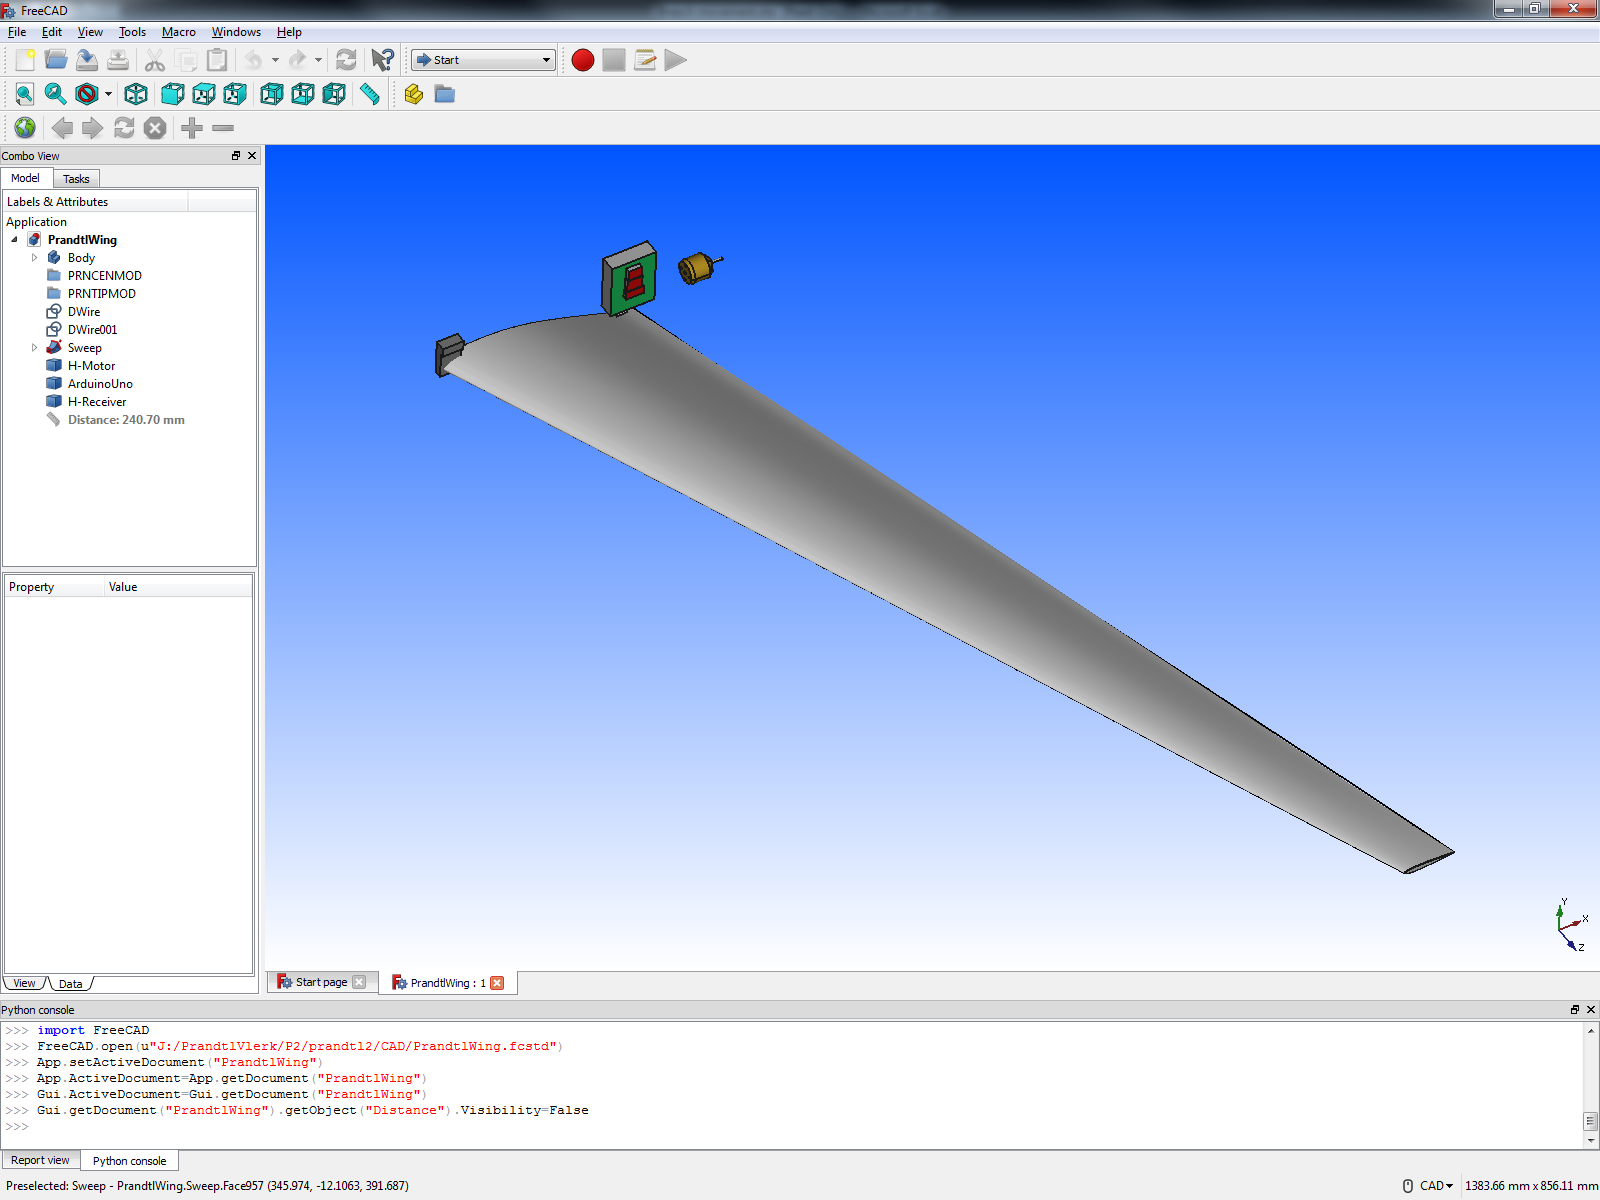
\includegraphics[width=0.7\linewidth]{Pictures/Prandtl2FreeCAD.png}
\end{figure}

\end{frame}


\begin{frame}
\frametitle{FEM}

FreeCAD Calculix FEA model of the Prandtl wing

\begin{figure}
        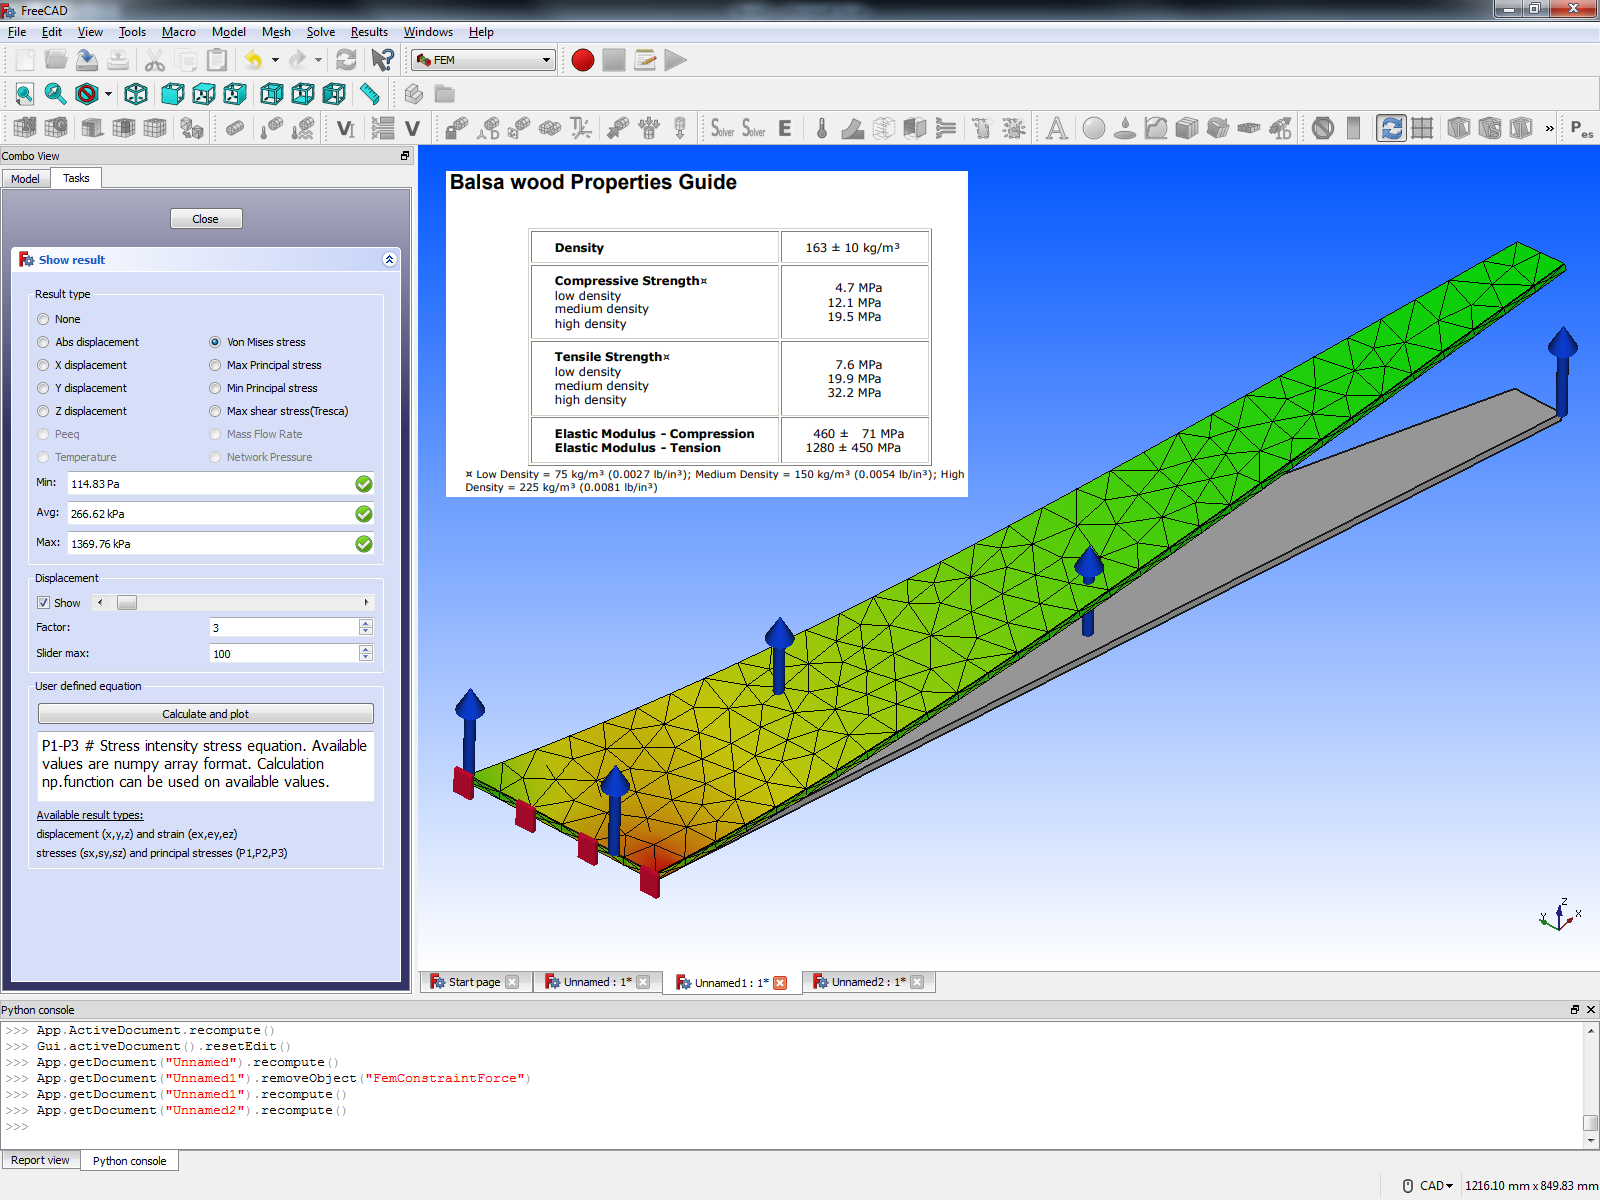
\includegraphics[width=0.7\linewidth]{Pictures/Prandtl2FreeCAD_FEM.png}
\end{figure}


\end{frame}

\begin{frame}
\frametitle{OpenFoam}

Blended wing body CFD analysis results from OpenFoam

\begin{figure}
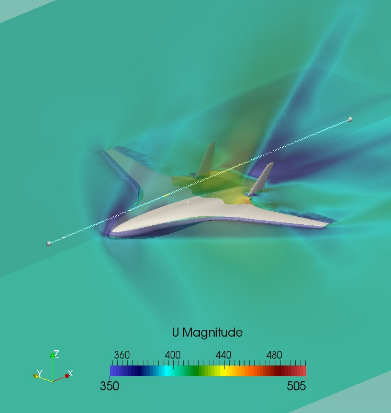
\includegraphics[width=0.4\linewidth]{Pictures/OpenFoamBWB.png}
\end{figure}

\end{frame}



\begin{frame}
\frametitle{Project Chrono}

A rover analyzed for rigid body dynamics with Project Chrono

\begin{figure}
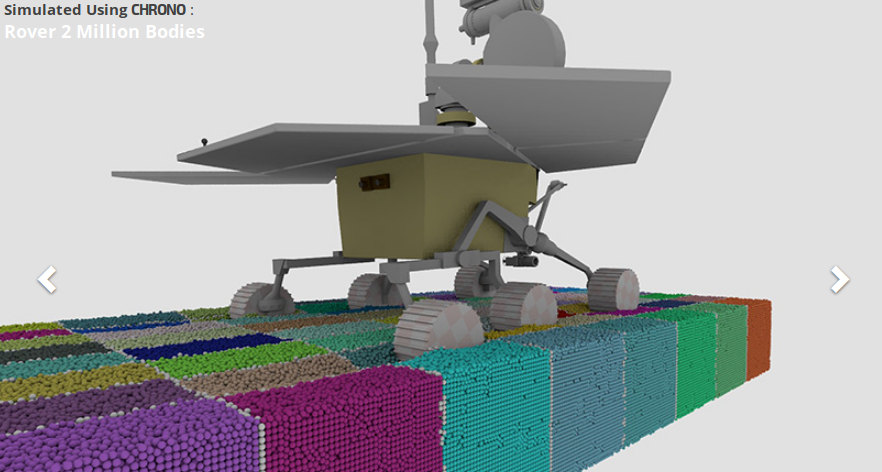
\includegraphics[width=0.8\linewidth]{Pictures/ProjectChronoRover.png}
\end{figure}

\end{frame}


\begin{frame}[fragile] % Need to use the fragile option when verbatim is used in the slide
\frametitle{Python}
$$ 
\sum_{n=1}^\infty A_n \sin(n \theta) \bigg(  \sin(\theta) + \frac{n C_{l \alpha} c}{8 s} \bigg) = \frac{C_{l \alpha} c}{8 s} \sin(\theta) (\alpha_\infty + \alpha_{geo} - \alpha_0) \qquad 
$$
\begin{example}[Lifting Line Code]
\begin{verbatim}
a = np.zeros([spanstations, nFourier])
for m in range(a.shape[0]): # rows
    for n in range(a.shape[1]): # columns
        a[m,n] = sin((n + 1)*theta[m])*(sin(theta[m]) 
        + (n + 1)*cla*c/(8*s))

b = np.zeros([spanstations])
for m in range(b.shape[0]): # rows of column vector
    b[m] = ((cla*c)/(8*s))*sin(theta[m])*(alfainf + 
    alfageo - alfazero)
x = np.linalg.solve(a, b)
\end{verbatim}
\end{example}

\end{frame}


\begin{frame}[fragile] % Need to use the fragile option when verbatim is used in the slide
\frametitle{Git}

\begin{example}[Updating a repository]
\begin{verbatim}
>>git add .
>>git commit -m "Update the presentation"
>>git push origin master
\end{verbatim}
\end{example}

\end{frame}



\section{FOSS philosophy}

%------------------------------------------------

\begin{frame}
\frametitle{Philosophy of Free Open Source Software (FOSS)}

\begin{itemize}
\item Free Open Source Software (FOSS) has some of its roots with the Free Software Foundation (started life with students from MIT), responsible for emacs

\item FOSS does in part democratize software and makes it transparent for everyone to use and edit with very few restrictions.
        
\item Free means not only `at zero cost', but also liberated (\emph{libre}) in the sense that it may be changed and distributed with little or no restriction
        
\item The implication of libre software is that it enables innovation by lowering the barriers to entry and standardizing methods all across the globe.
        
\item This might not seem very important at face value, but it has great consequences that have not been fully realized yet.
                
\end{itemize}


\end{frame}


\begin{frame}
\frametitle{Philosophy of FOSS}

The fact that libre software is available at no cost or lag (the time it takes to release software) has the following consequences:

\begin{itemize}
\item Skilled engineers that previously had little or no access to high end engineering software are now free to innovate
\item Libre software allows proper scaling to be possible, meaning that the number of engineers that can work on a problem is now only limited by the number of engineers you can find and not by license restrictions
\end{itemize}

\end{frame}


\begin{frame}
\frametitle{Philosophy of FOSS}

\begin{itemize}
\item The scaling of the engineering profession will have an exponential effect on innovation
\item It enables engineers to use complexity to their advantage since these packages enables execution of more complex analyses rapidly
\item Libre software provide a way of levelling the playing field with respect to engineering input costs, although it put a premium on skills, since engineers using it usually need more knowledge than the average user of paid software, since there is less technical support.
\item Software development can happen in parallel on a 24/7 basis with contributors from anywhere.  This is facilitated by tools like Git.
\end{itemize}

\end{frame}


%------------------------------------------------

%------------------------------------------------

\begin{frame}
\frametitle{Philosophy begin FOSS}

\begin{itemize}
\item The scaling effect of libre software is not as immediately apparent as it should be.  Let us explain by means of an analogy.  Let us examine a common system of metrology such as the metric system or the imperial system.
\item Up to 1920's many countries had different definitions of an inch.
\item Gauge blocks were invented in 1896 by Swedish machinist Carl Edvard Johansson.  To a large degree these gauge blocks standardized the industrial inch and also could be used for the metric system.
\item The gauge blocks made it possible for different machine shops, companies and indeed countries to have standard references of measurement.
\item This enables a global scalable manufacturing system.  Lego blocks made in Chech republic fits onto blocks made in the U.S. and not only that, they fit onto blocks made thirty years ago.
\item You can manufacture more, quicker than ever before at higher quality.        
\end{itemize}


\end{frame}



\begin{frame}

\frametitle{Metric gauge blocks}

Metric gauge blocks from Wikipedia:
\begin{figure}
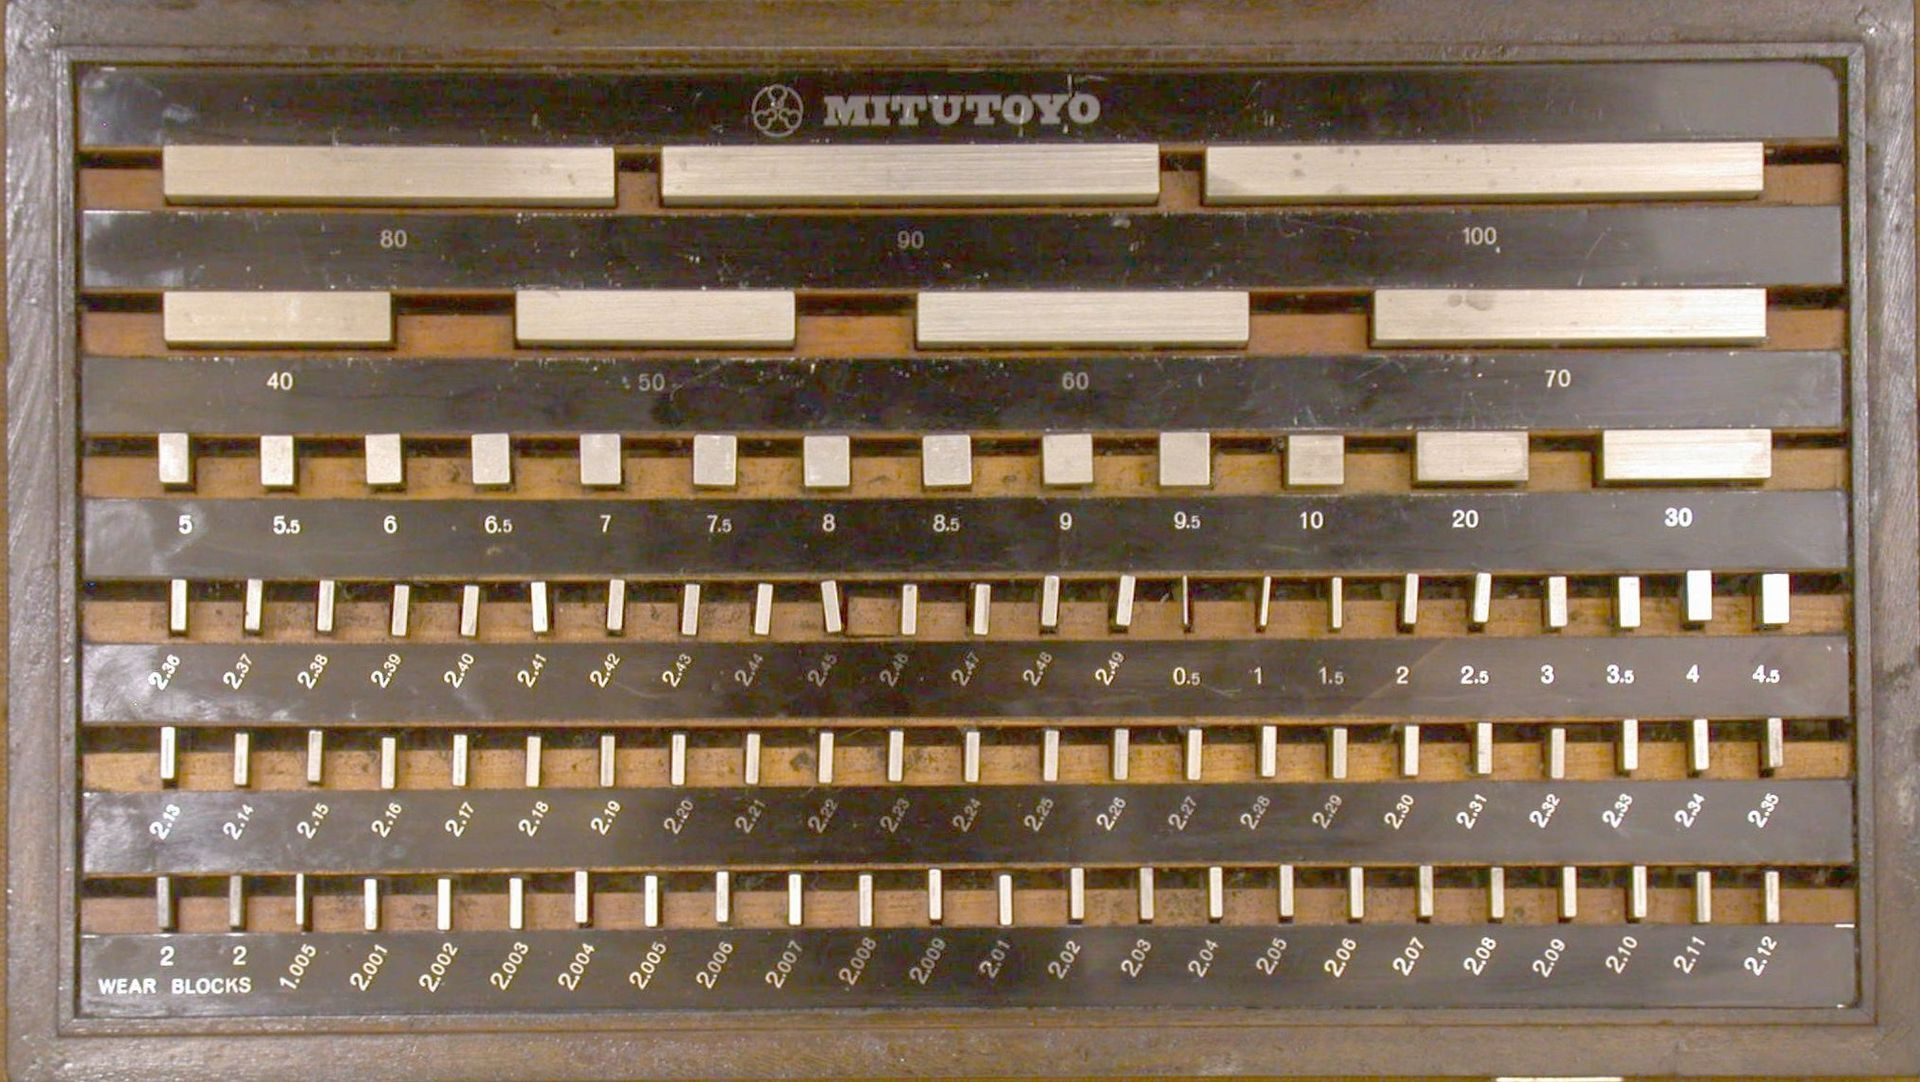
\includegraphics[width=0.8\linewidth]{Pictures/GaugeBlockMetricSet.jpg}
\end{figure}
\end{frame}


%------------------------------------------------


\begin{frame}
\frametitle{Philosophy begin FOSS}

\begin{center}
        FOSS is the software equivalent of gauge blocks
\end{center}

\begin{itemize}
\item All engineers in the world have the opportunity to use standard and benchmarked methods that have taken thousands of hours to develop.
\item They can share their ideas globally and scale on a level that has never been seen before.
\item All this without sacrificing flexibility, since standard methods can be forked and custom developed (while possibly later standardizing itself).  All the while the body of tools can grow.
\end{itemize}

\begin{center}
        You can analyze and engineer more products, quicker than ever before at higher quality.
\end{center}

\end{frame}


\begin{frame}
\frametitle{Philosophy begin FOSS}

\begin{itemize}
\item Gauge blocks standardized measurement and brought metrology out into the open.  This meant that specialized knowledge was not limited to companies or in a previous time, guilds.

\item Similarly libre software brings advanced analysis to any engineer willing to try and use the software.  It is now not limited to companies (in essence macro guilds) with large software budgets.

\item Standardization increased the gross product of manufacturing immensely over the last century leading to great prosperity for the entities that embraced it.

\item Libre software has the possiblility of providing just such a platform for innovation to scale exponentially.  Also with the accompanying properity and increase in gross product.
This will be aided by collaborative platforms such as Github that facilitates the large scale sharing of information, methods and contact between engineers.

\item Thus facilitating the free movement of ideas, intellectual (and consequently monetary) capital and contact between persons.

\end{itemize}

\end{frame}


\begin{comment}
Insert comments here
\end{comment}





\section{The engineering (r)evolution}

%------------------------------------------------

\begin{frame}
\frametitle{Mechanical/Aeronautical Engineering as coding discipline}

The lines are blurring between engineering and software coding.

\begin{itemize}
\item in FreeCAD a whole component can be constructed using python commands.  The versions of the CAD document can be controlled by Git, since the script file is a text file
\item Structural analysis calculations in a python notebook is a text file 
\item FEA runs produce large amounts of data stored in databases - requires programming to query and analyze further
\item Therefore adopt software methodologies for  engineering projects, such as agile project management
\end{itemize}

All text files are version controlled with git - another software tool

\end{frame}


%------------------------------------------------

%------------------------------------------------

\begin{frame}
\frametitle{Evolutionary aspects of innovation}

Evolutionary aspects and developmental aspects of software
\end{frame}


\begin{comment}
Verspreiding van sagteware
Kommersiële sagteware gestop deur koste en lisensies maar gehelp deur vriendelikheid en aggressiewe bemarking

Oopbron is onvriendelik en moeilik dog kragtig maar het oneindige prossesserings vermoë.

Die begin van video tutoriale, self dokumentasie en die internet en moontlike bemarking deur entoesiaste kan dalk die nadele oorkom. Ook platforms soos github. 

Dit is twee konsepte wat meeding om genetiese geskiktheid. Die uitkoms sal heel moontlik fraktaal wees en gekonsentreerd met wenner oorheers alles effekte.

Die belangrikste faktor is egter nie sagteware nie maar die beperkings op innovasie en hier styg oopbron sagteware uit. Dit strem glad nie innovasie nie en moedig dit aan. Vir hierdie rede maak dit sin om die oopbron tegnologie te ondersteun. Skaaleffekte van innovasie is belangriker omdat dit lei tot meer ontwikkeling en moontlike alhoewel nke gewaarborgde gepaardgaande welvarendheid.

Die nodigheid van 'n raamwerk kan nie onderskat word nie. Dit is wat platforms soos github gee. Dit wys groepe hoe om saam te werk en te werk tot 'n gemeenskaplike doel. Dit kan mega skaal groepe wat groter is as maatskappye mobiliseer en fokus. Die afwesigheid van goeie raamwerke kan verduidelik waarom IOT en tuis solar vir kragopwekking nog nie plaaslik posgevat het nie. Indien 'n goeie metafoor en raamwerk vir IOT en PLM en mikro grids vir kragopwekking daargestel kan word kan dit lei tot sukses.

Die belangrikheid van desentraliseerde organisasie moet hier onderstreep word. Dit is hardnekkig en iets anders as die hedendaagse sentralisasie wat heel moontlik nou 'n plato bereik het. Desentraliseerde organisasie was nooit werklik moontlik nie voor die konnektiwiteit wat nou beskikbaar is. 'n Platform soos tipies op 'n web implementasie maak dit moontlik. Soos bv 'n blockchain van kragopwekkking.

\end{comment}




%------------------------------------------------

%------------------------------------------------

\begin{frame}
\frametitle{Examples of evolutionary restrictions for engineering}

Explain how tailless aircraft evolve

Tailless aircraft have lagged significantly behind aircraft with a horizontal tail.  This is so severe that it is estimated that 10 times more development is now required to field a competitive tailless design when compared with a tailed design.

Much of the the performance of the tailless concept rests on the performance of the often reflexed airfoil of the aircraft.  In order to be competitive tailless aircraft also require laminar airfoils such as their tailed competitors.  But reflexed laminar profiles are extremely difficult to develop.  

Developing airfoil profiles requires many windtunnel hours and a littany of CFD and potential flow calculation runs.  The development of airfoils have been described as an evolutionary process and genetic algorithms have even been suggested in the past to develop them.
So imagine how restrictive it would be if the number of generations or iterations of an airfoil would be limited by not executing as many CFD runs as possible.
This happens in two ways since licenses would restrict the number of computers and engineers that would be working on the airfoil.  Furthermore it restricts capital investment in this concept since resources are diverted to expensive software costs.  
The diversion of capital resources to software further restricts the number of engineers that would be working on the problem.

This is a specific example for airfoils but this kind of restriction would be a similar barrier to all innovation.  
Furthermore the establishment of a license structure leads to a silo approach to product design, where certain departments keep the analysis tools in neat silos and preventing the innovation enabling tools to spread to other parts of an organization or innovatory clan.

\end{frame}

\begin{comment}
Tailless aircraft have lagged significantly behind aircraft with a horizontal tail.  This is so severe that it is estimated that 10 times more development is now required to field a competitive tailless design when compared with a tailed design.

Much of the the performance of the tailless concept rests on the performance of the often reflexed airfoil of the aircraft.  In order to be competitive tailless aircraft also require laminar airfoils such as their tailed competitors.  But reflexed laminar profiles are extremely difficult to develop.  

Developing airfoil profiles requires many windtunnel hours and a littany of CFD and potential flow calculation runs.  The development of airfoils have been described as an evolutionary process and genetic algorithms have even been suggested in the past to develop them.
So imagine how restrictive it would be if the number of generations or iterations of an airfoil would be limited by not executing as many CFD runs as possible.
This happens in two ways since licenses would restrict the number of computers and engineers that would be working on the airfoil.  Furthermore it restricts capital investment in this concept since resources are diverted to expensive software costs.  
The diversion of capital resources to software further restricts the number of engineers that would be working on the problem.

This is a specific example for airfoils but this kind of restriction would be a similar barrier to all innovation.  
Furthermore the establishment of a license structure leads to a silo approach to product design, where certain departments keep the analysis tools in neat silos and preventing the innovation enabling tools to spread to other parts of an organization or innovatory clan.

\end{comment}




\begin{frame}
\frametitle{Evolutionary aspects of FOSS example}
Bird in captivity born with prantl versus bird free born with prantl. Based on luck which is born free.

Bird mates in air therefore is more fit with prandtl and has many offspring. Goes on to be dominant. 

Captive bird dies.


Free software and open source spreads ideas and makes mutation and natural selection more possible. Especially advatageous in industries where capital is not readily available.
\end{frame}

%------------------------------------------------



\section{Open Source and currency and patents}


\begin{frame}
\frametitle{FAQ:  Show me the money}

Most common FAQ with open source:  

\begin{center}

\emph{How do you make money with open source?}


\includegraphics[width = 0.5\textwidth]{Pictures/showmethemoney.jpg}
\end{center}
\end{frame}


\begin{frame}
\frametitle{Reason for the question}

\begin{center}

This question asked is because most people have a fundamental lack of understanding of currency.

\end{center}
\end{frame}


\begin{frame}
\frametitle{The function of money}

Money is simply a means of exchanging goods and services on an equal value basis. Money is created and the flow that results from the exchanges results in economic growth prosperity.

\end{frame}

\begin{frame}
\frametitle{Fractional banking}

\begin{itemize}
\item Personal finance is done on a zero sum game basis (leads to most misunderstanding)
\item With economic growth (as with innovation) the system is not zero sum game
\item The example is fractional banking
\end{itemize}

\end{frame}


\begin{frame}
\frametitle{Fractional banking}

\begin{itemize}
\item Bank accepts deposits (noble metal in the old days)
\item Depositors get paper (or electronic) proof of the deposits
\item This proof now gets traded instead of the actual deposit
\item Bank realises it does not need to hold 100\% of deposits
\item Bank starts creating money by issuing loans
\item This is OK as long as there is no run on the bank and the loans are not defaulted
\item Economic growth has happened
\end{itemize}

\end{frame}

\begin{frame}
\frametitle{Back to engineering and innovation}

\begin{itemize}
\item The cost of hardware is coming down rapidly 
\item Most expensive part is the intellectual firepower needed to understand and develop products that in turn create prosperity
\item The cost of the innovation cycle is only around 20\% of the full product development cycle (eg. aircraft prototype versus production aircraft)
\item Therefore most important part of the 20\% will be intellectual capital
\item This is even more important when most of development will be done in a simulation environment
\item Consequently, although hardware is expensive, it is not the blocking point for innovation
\end{itemize}

\end{frame}


\begin{frame}
\frametitle{Intellectual capital}

\begin{itemize}
\item So if you create software to analyze some product and you open source it you have created intellectual currency - you have created capital by making a loan to the technical community
\item Now some other person uses your software to make a hardware design for which you did not have the expertise and that person open sources that
\item That person now created more intellectual currency (essentially repaying the debt) that can now be used to develop ever more products
\item Intellectual capital has been created and growth has happened that leads to innovation and prosperity
\item If the cycle of open sourcing is broken, this amount to a default on the intellectual capital debt
\end{itemize}

\end{frame}


\begin{frame}
\frametitle{If money had been used}

\begin{itemize}
\item Pay for software (in hard currency) you use to analyze your concept 
\item Then pay for hardware to build your product that might or might not be successful  
\item Resulting much more expensive product that few people can afford
\item The use of money as a basis for exchange in this case is hysteresis which was not necessary in the first place
\end{itemize}

\end{frame}


\begin{frame}
\frametitle{Use money appropriately}

\begin{itemize}
\item Why use money as a tool for exchange of intellectual capital when it can be exchanged directly
\item It is possible for ideas, designs and software to be exchanged without the resulting loss of that information to the giver (see later expansion of this idea)
\item Resulting much more expensive product that few people can afford
\item You are therefore not poorer by open sourcing but instead you become an investor in intellectual capital
\end{itemize}

\end{frame}


\begin{frame}
\frametitle{Use money appropriately}

\begin{itemize}
\item We are essentially not applying money correctly by using it to pay for engineering resources sometimes (especially during concept phases)
\item Money should not be the end. But rather should only be used as a tool for exchange where exchange is not otherwise possible
\item Using money for exchanges where it is not required shows fundamental lack of understanding. And causes enormous losses
\end{itemize}

\end{frame}


\begin{frame}
\frametitle{Overspending}

\begin{itemize}
\item Intellectual overspending is also possible 
\item Example:  A person that only works on math problems or interesting programming problems fails to gather food or money to buy food and now has a survival problem
\item Equally only working on open source software will lead to poverty
\item Caveat:  An important balance has to be struck with intellectual capital as well
\item The open source practioners should still value and sell their time
\end{itemize}

\end{frame}


\begin{frame}
\frametitle{Overspending Example}

\begin{itemize}
\item The cautionary tale of Chinese great leap forward is applicable to open sourcing 
\item Millions of people stopped farming for food and started only making steel without making a deal to exchange some of the steel for food
\item  This shows a fundamental lack of understanding of an economy.  The exchange is important. 
\item It might have been OK, had some people still farmed while others made steel
\item But this did not happen.  Millions starved and insult to injury was that the steel was of poor quality.
\item Similarly dropping everything you do to to pursue open source would be folly
\end{itemize}

\end{frame}


\begin{frame}
\frametitle{Preventing Intellectual Overspending}

\begin{itemize}
\item Development of several small tools are important. This is antifragile. Because it prevents a centralized overexpenditure of intellectual capital.
\item Small tools part of libraries developed in a decentralized way also enables scaling.  It enables networks of people to spend small amounts of intelectual capital.
\item  Large pieces of paid software are an example of intellectual overspending and achieve the opposite.  They centralize the several small tools into one.  Leading to centralized control and the accompanying fragility of concentration.  Now engineers are concentrated and are vulnerable because they are totally reliant on money as an exchange for their services/software.  Inefficiencies result from this.
\end{itemize}

\end{frame}


\begin{frame}
\frametitle{Free money:  You pick it up it's yours}

\begin{itemize}
\item Essentially NASA gave us (non US citizens) free intellectual capital by open sourcing the Prandtl wing and their technical reports server
\item Or maybe they just invested their government's tax revenue semi wisely
\end{itemize}

\end{frame}  



\begin{comment}

Opensource engineering most faq is how do you make money with open source. This is because most people have a fundamental lack of understanding of currency.

It is only a means of exchanging goods and services on an equal value basis. Money is created and the flow that results from the exchanges results in prosperity.  Show example of fractional reserve banking.

So now in an engineering economy the cost of hardware is coming down quickly. Most expensive part is the intellectual firepower needed to understand and develop products that in turn create prosperity. 

So if you create software to analyze some product and you open source it you have created intellectual currency. Now some other person uses your software to make a hardware design for which you did not have the expertise and that person open sources that. He or she now created more intellectual currency that can now be used to develop ever more products. 

Lets see how money would have been used. Pay for software then pay for hardware and a resulting much more expensive product that few people can afford. The money in this case is hysteresis which was not necessary in the first place. 

You are therefore not poorer by open sourcing but instead you become an investor in intellectual capital. 

We are essentially not applying money correctly by using it to pay for engineering resources sometimes.

Money should not be the end. But rather should only be used as a tool for exchange where exchange is not otherwise possible. Using money for exchanges where it is not required shows fundamental lack of understanding. And causes enormous losses.


If you intellectually overspend like when you only work on math problems and not get food then you have a problem because now you have to get money for your software to provide food. 

So an important balance has to be struck with intellectual capital as well. Example is the Chinese great leap forward where people stopped making food and started only making steel withou making a deal to exchange some of the steel for food. Again showing fundamental lack of understanding of an economy.  The exchange is important. The ways of exchanging is only important in facilitating.

Similarly the development of several small tools are important. This is antifragile. Because it prevents a centralized overexpenditure of intellectual capital.  Large pieces of paid software are an example of this.  They centralize the several small tools into one.  Leading to centralized control and the accompanying fragility of concentration.  Now engineers are concentrated and are vulnerable because they are totally reliant on money as an exchange.  Inefficiencies result from this.


Essentially NASA gave us intellectual capital by open sourcing the Prandtl wing.
\end{comment}





\begin{frame}
\frametitle{FAQ:  If I open source then is my idea is lost}

Second most common FAQ with open source:  

\begin{center}

\emph{How do you patent your idea with open source?}

\end{center}
\end{frame}


\begin{frame}
\frametitle{Patents, ideas and concepts are not zero sum game}

\begin{center}

When someone shares an idea, concept or method (this extends to software and CAD) with someone else then the person that shared the information still possesses the information.  Information is not destroyed by transmission.  This makes it fundamentally different to commodities and property, where once ownership is transferred the original owner does not possess the commodity or property.  As such information is not tradeable.

\end{center}
\end{frame}

\begin{frame}
\frametitle{This is not a new idea}

\begin{center}

Thomas Jefferson to Isaac McPherson, 13 August 1813:

\emph{if nature has made any one thing less susceptible, than all others, of exclusive property, it is the action of the thinking power called an Idea; which an individual may exclusively possess as long as he keeps it to himself; but the moment it is divulged, it forces itself into the possession of every one, and the reciever cannot dispossess himself of it. it’s peculiar character too is that no one possesses the less, because every other possesses the whole of it. he who recieves an idea from me, recieves instruction himself, without lessening mine; }

\end{center}
\end{frame}


\begin{frame}
\frametitle{This is not a new idea}

\begin{center}

Thomas Jefferson to Isaac McPherson, 13 August 1813:

\emph{... as he who lights his taper at mine, recieves light without darkening me. that ideas should freely spread from one to another over the globe, for the moral and mutual instruction of man, and improvement of his condition, seems to have been peculiarly and benvolently designed by nature, when she made them, like fire, expansible over all space, without lessening their density in any point; and like the air in which we breathe, move, and have our physical being, incapable of confinement, or exclusive appropriation. }

\end{center}
\end{frame}


\begin{frame}
\frametitle{Story time:  A Patent on the motor vehicle}

\begin{itemize}
\item The Association of Licensed Automobile Manufacturers (ALAM) used the patent on the motor vehicle to force manufacturers pay a 5\% royalty on all cars produced
\item They had some degree of control of who was allowed to produce cars
\item They denied the franchise to Henry Ford
\item Ford challenged and eventually beat ALAM in court to win the right to produce motor vehicles
\item Patents nearly negatively influenced the mass production of vehicles
\item It therefore nearly denied many people the freedom of movement
\item Henry Ford did NOT patent his moving assembly line.  The stationary assembly line was however patented by Ransom Olds in 1901, long before the Ford factories.
\end{itemize}

\end{frame}


\begin{frame}
\frametitle{Joke time:  A Patent on flight}

From Wikipedia:

\begin{itemize}
\item The Wright brothers patent war stalled development of the U.S. aviation industry 
\item Airplane development in the United States fell so far behind Europe that in World War I American pilots were forced to fly European combat aircraft, instead
\item After the war began, the U.S. Government pressured the aviation industry to form an organization to share patents
\end{itemize}

\begin{center}
Joke:  Would they have told birds to stop flying because they didn't pay their royalties?
\end{center}
\end{frame}


\begin{frame}
\frametitle{Who owns the idea}

\begin{center}

The following points arise:

\begin{itemize}
\item Ideas are not tradeable like commodities
\item The fairness of exclusive rights to an idea is dubious
\item Patenting the laws of physics seems unintelligent
\item International law provides limited protection for patents in any event
\item Patents probably are not helpful to innovation
\item The question is not whether you should patent, but rather should you not work harder to get the first mover advantage (this is arguably more valuable)
\end{itemize}

\end{center}
\end{frame}


\section{Conclusions}

\begin{frame}
\frametitle{Conclusions}

The following conclusions are personal opinions:

\begin{itemize}
\item Open source tools and platforms have an important role to play - especially for aircraft that require so much analysis
\item Open source tools have reached a level of maturity that is useful for some industrial application - they are not toys any more
\item Network effects are important for innovation
\item Open hardware and software will accelerate economic activity and prosperity through value and intellectual capital creation
\item Engineering is coding
\item Information should be exchanged without the use of currency to prevent hysteresis losses
\item Exclusive ownership of ideas is probably a barrier to innovation
\end{itemize}
\end{frame}


\begin{frame}
\frametitle{References}
\footnotesize{
\begin{thebibliography}{99} % Beamer does not support BibTeX so references must be inserted manually as below

\bibitem{PrandtlBowers} Albion H. Bowers, and Oscar J. Murillo (2016) On Wings of the Minimum Induced Drag:  Spanload Implications for Aircraft and Birds, NASA/TP-2016-219072
\bibitem{PrandtlPatent} US Patent 9,382,000 B1, July 5, 2016, Bowers et al.
\bibitem{omegataupodcastPrandtl} Markus Voelter (2017) omega tau podcast number 256 – Flight Research at NASA Armstrong, Part 1: Subscale, http://omegataupodcast.net/256-flight-research-at-nasa-armstrong-part-1-subscale/
\bibitem{Prandtl1921} Prandtl, L.  (1921)  Applications  of  modern hydrodynamics  to  aeronautics,  NACA  Report  No  116 (Washington, DC).
\bibitem{Prandtl1933} Prandtl L (1933) Über tragfl\"ugel kleinsten induzierten widerstandes. Zeitschrift für Flugtecknik und Motorluftschiffahrt, 1 VI 1933 (M\"unchen, Deustchland).
\bibitem{ModelFlightNASA} Joseph R. Chambers, Modelling Flight - The role of dynamically scaled free-flight models in support of NASA's aerospace programs, ISBN 978-0-16-084633-5.
\bibitem{NickelWohlfahrt} Karl Nickel and Michael Wohlfahrt, Tailless aircraft in theory and practice.


\end{thebibliography}
}
\end{frame}


%------------------------------------------------

\begin{frame}
\Huge{\centerline{The End}}
\end{frame}

%----------------------------------------------------------------------------------------

\end{document} 
